\documentclass{article}
\setcounter{tocdepth}{4} %Required to insert paragraph in TOC
\setcounter{secnumdepth}{4} %Required to insert paragraph in TOC

\usepackage{graphicx} % Required for inserting images
\graphicspath{ {./img/} }

\usepackage{blindtext}
\usepackage{titlesec}
\usepackage[dvipsnames]{xcolor}
\usepackage{geometry}
\geometry{
	a4paper,
	total={170mm,257mm},
	left=25mm,
	top=20mm,
}

\usepackage{adjustbox}
\usepackage{amsmath}
\usepackage{amssymb}
\usepackage{cancel}
\usepackage{caption}
\usepackage{subcaption}
\usepackage{titlesec}
\usepackage{float}
\usepackage{enumitem}
\usepackage{hyperref}
\usepackage{makecell}
\usepackage{chronology}

\setcounter{secnumdepth}{4}

\newcommand{\foo}{\hspace{-2.3pt}$\bullet$ \hspace{5pt}}

\titleformat{\paragraph}
{\normalfont\normalsize\bfseries}{\theparagraph}{1em}{}
\titlespacing*{\paragraph}
{0pt}{3.25ex plus 1ex minus .2ex}{1.5ex plus .2ex}

\title{Appunti Architettura dei Calcolatori Elettronici}
\author{Mattia Robuschi Caprara}
\date{}

\definecolor{CoverGreen}{RGB}{54,141,248}

\begin{document}
	
	\begin{titlepage}
		
		\pagecolor{CoverGreen}
		
		\vspace{25 mm}
		\begin{center}
			\large
			{\color{black}\textbf{Mattia Robuschi Caprara}} 
		\end{center}
		
		\begin{center}
			\huge
			{\color{black}\textbf{Architettura dei Calcolatori Elettronici}}
		\end{center}
		
		\vspace{45 mm}
		
		\begin{figure}[h]
			\centering
			\adjustbox{cfbox=white 5pt 0cm}{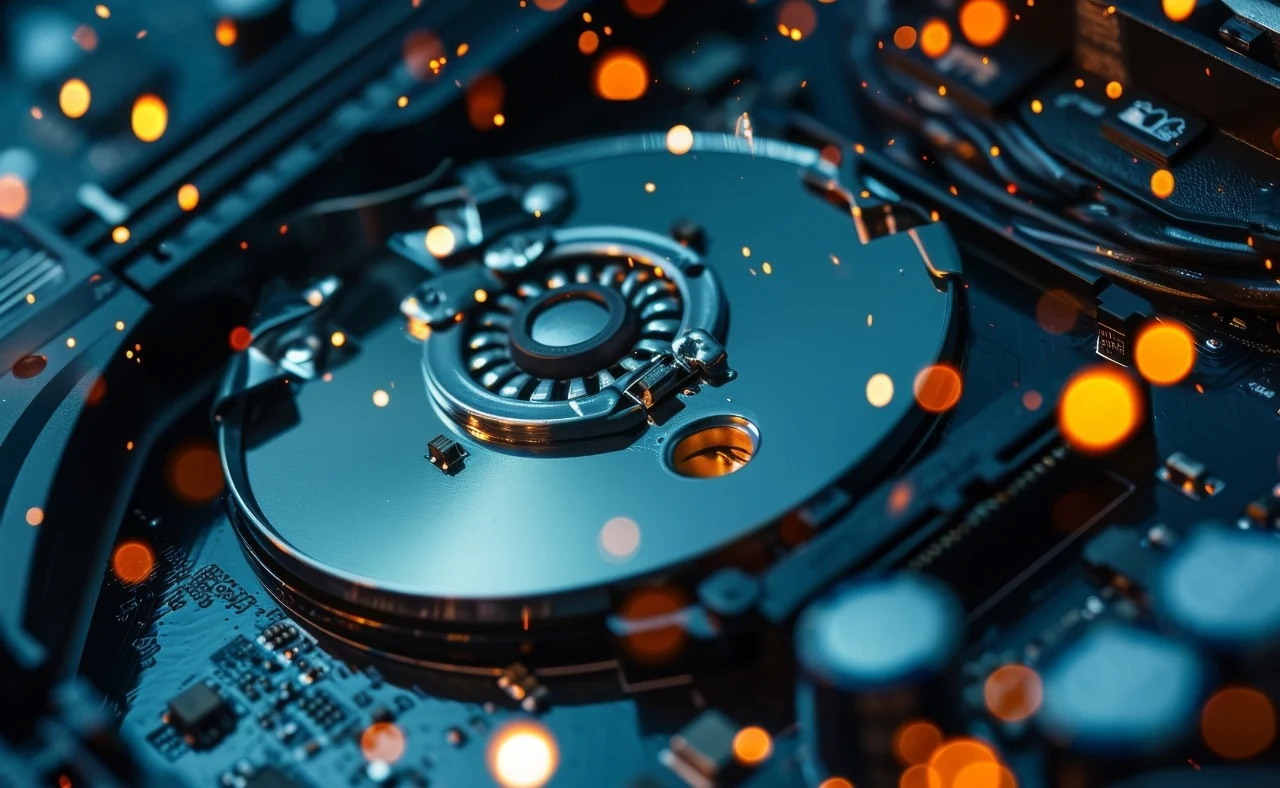
\includegraphics[scale=0.3]{0.cover.jpeg}}
			%\caption{Caption}
			\label{fig:cover}
		\end{figure}
		
		\thispagestyle{empty} 
	\end{titlepage}
	
	\newpage
	\pagecolor{white}
	\section*{Prefazione}
	\tableofcontents
	\newpage
	
	\section{Introduzione}
	\subsection{Cos'è un calcolatore elettronico}
	L’elaboratore o calcolatore elettronico svolge in automatico l’operazione
	di elaborare i dati a seconda delle istruzioni ricevute
	\begin{figure}[h]
		\centering
		\begin{subfigure}[b]{0.45\textwidth}
			\centering
			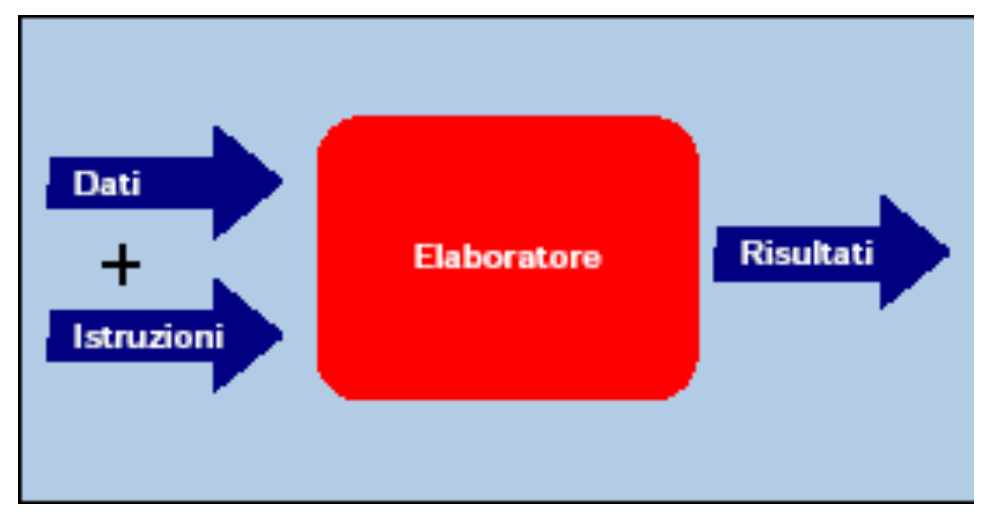
\includegraphics[width=\textwidth]{1.png}
			\caption{Schema 1}
			\label{fig:im-1}
		\end{subfigure}
		\hfill
		\begin{subfigure}[b]{0.45\textwidth}
			\centering
			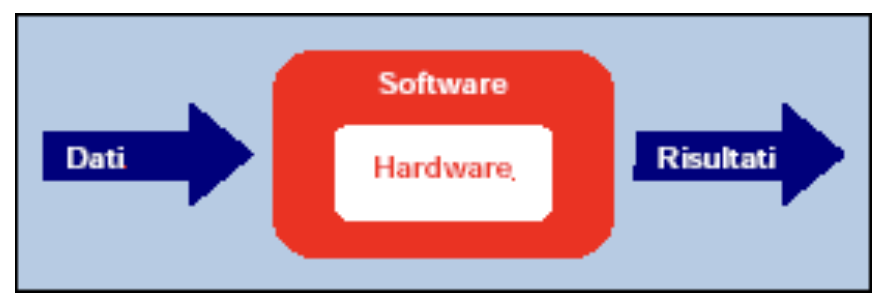
\includegraphics[width=\textwidth]{2.png}
			\caption{Schema 2}
			\label{fig:im-2}
		\end{subfigure}
		\caption{Schemi funzionamento calcolatore elettronico}
	\end{figure}
	\subsubsection{Algoritmi}
	Un algoritmo è un insieme di azioni (o istruzioni) che, eseguite secondo un ordine prestabilito, permettono di trovare il risultato cercato sulla base dei dati in ingresso.\\ \\
	Il calcolatore elettronico per risolvere un problema utilizza un algoritmo.\\ \\
	Il concetto di algoritmo è uno dei concetti di base dell'intera matematica: i più semplici ed antichi algoritmi sono le regole per eseguire le operazioni dell'aritmetica elementare, formulate dal matematico arabo medioevale Al-Khuwarizmi, da cui deriva appunto il nome di algoritmo.\\ \\
	Un computer non è altro che un rapidissimo esecutore di sequenze di istruzioni ovvero gli algoritmi.
	\subsubsection{Utilizzo dei calcolatori elettronici}
	Alcuni esempi di utilizzo di un calcolatore elettronico possono essere:
	\begin{itemize}
		\item Uno strumento di word processing
		\item Uno strumento di data analysis
		\item Un componente essenziale di robot, veicoli, strumenti di comunicazione, ecc...
		\item Uno strumento di controllo di sistemi complessi
		\item Uno strumento di progettazione CAD-CAM
		\item Uno strumento di gestione delle informazioni (Server)
	\end{itemize}
	\newpage
	\subsection{Funzionamento di un calcolatore}
	Un calcolatore elettronico deve svolgere 4 compiti principali:
	\begin{enumerate}
		\item Elaborazione (Calcolo)
		\item Memorizzazione
		\item Trasmissione
		\item Controllo
	\end{enumerate}
	\begin{figure}[h]
		\centering
		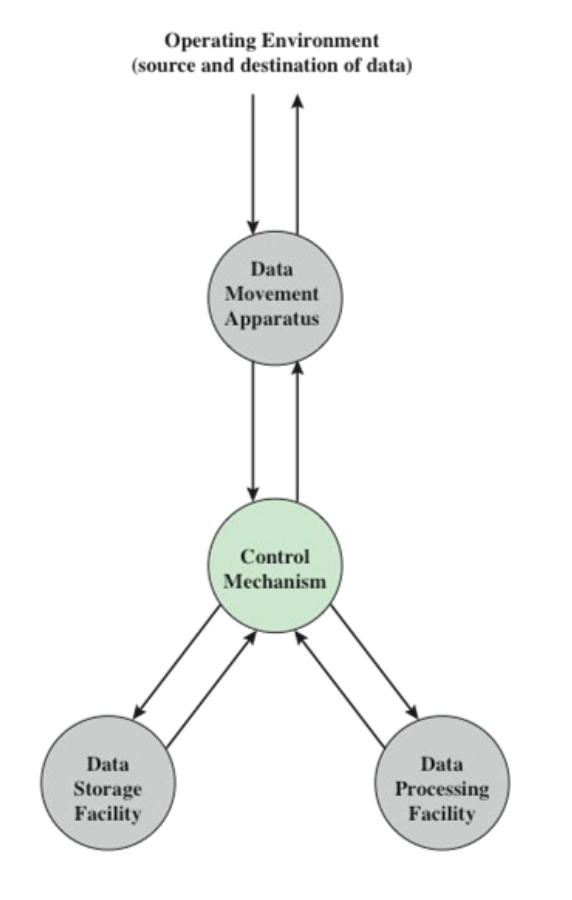
\includegraphics[scale=0.5]{3.png}
		\caption{Schema 2}
		\label{fig:im-3}
	\end{figure}
	Le 4 funzioni possono essere collegate approssimativamente a 4 componenti principali:
	\begin{itemize}
		\item CPU (Central Processing Unit), che a sua volta puù essere suddiviso in:
		\subitem Unità di controllo
		\subitem ALU (Unità Aritmetico-Logica)
		\subitem Registri (Generali o Dedicati)
		\subitem Interconnessioni
		\item Memoria
		\item Sistema di Memoria
		\item I vari BUS
	\end{itemize}
	\subsection{Storia dei calcolatori}
	I calcolatori hanno subito svariate evoluzioni durante il corso della storia:\\ \\
	\scalebox{1}{
		\begin{tabular}{r |@{\foo} l}
			$\rightarrow$ 1834 & \textbf{Analytical Engine (Babbage)} – primo “computer” digitale\\
			1946 & \textbf{ENIAC} (Electronic Numerical Integrator And Calculator)\\
			1951 & \textbf{UNIVAC-I} – primo calcolatore comm. – 250,000 \$ - 48 esemplari\\
			1952 & \textbf{IBM 701} (prima solo macchine da ufficio)\\
			1952 & \textbf{Macchina IAS di Princeton} (macchina di \textbf{Von Neumann})\\
			1962 & \textbf{IBM 709x} (primo calcolatore scientifico di discreta potenza)\\
			$\rightarrow$ 1964 & \textbf{IBM S/360} – primo tentativo di def. di architettura (Uno dei primi Mainframe)\\
			1964 & \textbf{CDC 6600} – primo supercalcolatore (poi Cray) (Uno dei primi Mainframe)\\
			1965 & \textbf{DEC PDP 8} – primo minicalcolatore (< \$20.000) – accum. a 8 bit\\
			1970 & \textbf{DEC PDP 11} – calcolatore a 16 bit, unico bus\\
			$\rightarrow$ 1971 & \textbf{CPU 4004} microprocessore (Intel) (sistema MCS-4) – a 4 bit\\
			1972 & \textbf{Intel 8008} – prima CPU a 8 bit (30 micros./istr.)\\
		\end{tabular}
	} \\
	\scalebox{1}{
		\begin{tabular}{r |@{\foo} l}
			$\rightarrow$ 1974 & \textbf{National PAC} – prima CPU single chip a 16 bit\\
			1974 & \textbf{Intel 8080} – seguito da Motorola MC6800 e Zilog Z80\\
			1974 & \textbf{Cray-1} – primo supercomputer vettoriale\\
			$\rightarrow$ 1978 & \textbf{Intel 8086} – primo processore di seconda generazione in grado di indirizzare oltre a 64kB \\ & – seguito da MC68000 e Z8000\\
			1978 & \textbf{DEC VAX} – riferimento per i mainframe futuri\\
			$\rightarrow$ 1979 & \textbf{Intel 8088} – processore a 8 bit con architettura interna a 16 bit (m = 16)\\
			1979 & \textbf{IBM 801} – primo processore RISC (32 bit)\\
			$\rightarrow$ Fine 70' & \textbf{IBM S/370} – compatibile con S/360\\
			$\rightarrow$ 1982 & \textbf{RISC I} – University of Berkley (In contrasto con CISC)\\
			$\rightarrow$ 1984 & \textbf{MC68020} – prima CPU a 32 con cache istruzioni integrata + MMU (m = 32)\\
			1985 & \textbf{MIPS} – University of Standford\\
			1985 & \textbf{Intel 80386} – CPU a 32 bit con MMU (Memory Management Unit) integrata\\
			1987 & \textbf{MC68030} – prima CPU con cache separate e MMU (32 bit)\\
			1989 & \textbf{MC68040} – prima CPU con anche FPU\\
			$\rightarrow$ 1989 & \textbf{Intel 80486} – cache integrata\\
			$\rightarrow$ Inizi 90' & \textbf{PowerPC} – architettura RISC, da unione IBM, Apple e Motorola\\
			$\rightarrow$ 1993 & \textbf{Pentium} – nuova architettura superscalare con \textbf{parallelismo esplicito}\\
			1995 & \textbf{Pentium Pro} – esecuzione speculativa, predizione salti, … \\
			1997 & \textbf{Pentium II} – tecnologia MMX (modifica ISA)\\
			1999 & \textbf{Pentium III} – istruzioni per la gestione della grafica 3D\\
			2000 & \textbf{Pentium 4} – istruzioni multimediali\\
			6/2001 & \textbf{Itanium Merced} – IA-64 congiunta Intel-HP – esperimento\\
			6/2002 & \textbf{Itanium 2 McKinley} – commerciale\\
			$\rightarrow$ 5/2005 & \textbf{Intel Pentium D (EE 840), AMD Athlon 64 X2} – architettura dual-core\\
			7/2006 & \textbf{Intel Core 2 Duo (Core microarch.)} – fine Pentium\\
			2008 & \textbf{Intel Core 2 Quad} – fino al Q9300 (2.4 GhZ, L2 6MB)\\
			2014 & \textbf{Intel Core i7 Extreme} – fino a i7-5960X (8 core,3.5 Ghz,L2 20MB)\\
		\end{tabular}
	}
	%\begin{chronology}[8]{1834}{1972}{100ex}[\textwidth]
		%\event{1834}{one}
		%\event{1946}{two}
		%\event{1953}{three}
	%\end{chronology}
	\subsection{Generazioni dei calcolatori}
	Un altro modo per visualizzare l'evoluzione dei calcolatori elettronici è tramite la suddivisione in generazioni, anche se queste potrebbero non essere del tutto precise.
	\subsubsection{Generazione 0 - Computer Meccanici}
	\paragraph{Analytical Engine}
	\subsubsection{Generazione 1 - Valvole}
	\paragraph{ENIAC}
	\paragraph{Architettura di Von Neumann}
	\paragraph{Architettura di Harvard}
	\paragraph{IAS Computer}
	\subsubsection{Generazione 2 - Transistor}
	\paragraph{Transistor}
	\paragraph{IBM 709x}
	\subsubsection{Generazione 3 - Circuiti Integrati}
	\paragraph{Circuiti integrati (SSI, MSI, LSI)}
	\paragraph{PDP-8}
	\subsubsection{Generazione 4 - Integrazione a grandissima scala}
	\paragraph{VLSI}
	\subsubsection{Generazione 5 - Computer avanzati}
	\subsection{Legge di Moore}
	\subsection{Seconda Legge di Moore}
	\subsection{Legge di Amdahl}
	\subsection{Parallelismo}
	\subsubsection{Supercalcolatori CM2}
	\subsubsection{MMX poi SSE (SIMD)}
	\subsubsection{Cluster}
	\subsubsection{Multicore}
	
\end{document}